% -----------------------------
% Корневой файл (компиляция с него)
% -----------------------------

\documentclass[12pt, russian, indentheadings]{report}

%\input{package_conf.tex}
\usepackage[utf8]{inputenc}
\usepackage[russian]{babel}
\usepackage{amsmath, amssymb}
\usepackage{graphics}
\usepackage{graphicx}
\usepackage{tabularx}


\begin{document}
%\selectlanguage{russian}

%\renewcommand{\captionlabeldelim}{~---}
\renewcommand{\labelitemi}{---}
\renewcommand{\labelitemii}{---}
\renewcommand{\labelitemiii}{---}
\renewcommand{\figurename}{Рисунок}
\renewcommand\thefigure{\Alph{part}.\arabic{chapter}.\arabic{figure}}
\renewcommand\thetable{\Alph{part}.\arabic{chapter}.\arabic{table}}
\frenchspacing

\title{Задача дробного переноса}

%\tableofcontents

\chapter{Постановка задачи}
Необходимо решить уравнение переноса с дробной производной Римана-Лиувилля по времени:
\begin{equation}
	\begin{cases}
		D^\alpha_t c + (uc)_x = f(x,t)\\
		\left.J^{1-\alpha}_tc\right|_{t=0} = \phi(x)\\
		\left.c\right|_{x=0}=\psi(t)
	\end{cases}
\end{equation}

Простейший случай предполагает $u=const$.

\chapter{Аналитическое решение}
\section{Задача без источника с постоянной скоростью}

Для первого приближения принимается упрощение: скорость переноса $u(x,t)$ принимается за постоянную

\begin{equation}
	u(x,t) \equiv u = const,
\end{equation}
также считаем задачу без источников $f(x,t)\equiv0$, тогда система (\label{eq:def_0}) принимает вид

\begin{equation}
	\label{eq:an_0}
	\begin{cases}
		D^\alpha_t c + uc_x = 0\\
		\left.J^{1-\alpha}_tc\right|_{t=0} = \phi(x)\\
		\left.c\right|_{x=0}=\psi(t)
	\end{cases}
\end{equation}

Тогда применяем преобразование Лапласа $L_t(f(t))$ к главному уравнению системы, учитывая свойство
\begin{equation}
	L_t(D^\alpha_tf(t))(s) = s^\alpha f^* - \left. I^{1-\alpha}_tf \right|_{t=0},
\end{equation}
и получаем
\begin{equation}
	s^\alpha c^*(x,s) - \phi(x) + u c^*_x(x,s) = 0,
\end{equation}
\begin{equation}
	c^*(x,s) = \frac{\phi(x)}{s^\alpha + u D_x}.
\end{equation}
С использованием свойства
\begin{equation}
	L_t(e^{\lambda t}_{\alpha}) = \frac{1}{s^\alpha-\lambda}
\end{equation}
где
\begin{equation}
e^{\lambda t}_{\alpha} =
t^{\alpha - 1} E_{\alpha, \alpha}(\lambda t^{\alpha}) =
\sum_{k = 0}^{\inf}\frac{\lambda^k t^{(k+1)\alpha - 1}}{\Gamma(k\alpha + \alpha)}
\end{equation}
Тогда получаем решение
\begin{equation}
	c(x,t) = e^{utD_x}_{\alpha} \phi(x),
\end{equation}

\begin{equation}
	c(x,t) = \sum_{k = 0}^{\inf}\frac{(-u)^k t^{(k+1)\alpha - 1}}{\Gamma(k\alpha + \alpha)} D^k_x \phi(x),
\end{equation}


\chapter{Численное решение}
\section{Преобразования системы}
Численный расчет исзодного уравнения проблематичен, так как в момент $t=0$ в уравнении присутствует интегрируемая особенность (сингулярность). Поэтому производятся преобразование:
\begin{equation}
	w = J^{1-\alpha}_t c - \phi(x),
\end{equation}
\begin{equation}
	c = D^{1-\alpha}_t \left( w + \phi(x) \right)
	= D^{1-\alpha}_t w + \phi(x) \frac{t^{\alpha - 1}}{\Gamma(\alpha)}
\end{equation}


Тогда система принимает вид

\begin{equation}
	\begin{cases}
		w_t + u \left( D^{1-\alpha}_t \left( w + \phi\left(x\right) \right) \right)_x = f(x,t)\\
		\left.w\right|_{t=0} = 0\\
		\left.D^{1-\alpha}_t \left( w + \phi(x) \right) \right|_{x=0} = \psi(t)
%		= \psi(t) - \phi(0) \frac{t^{\alpha - 1}}{\Gamma(\alpha)}
	\end{cases}
\end{equation}
или
\begin{equation}
	\label{eq:num1}
	\begin{cases}
		w_t + u \left( D^{1-\alpha}_t w\right)_x
		= f(x,t) - u \phi_x\left(x\right)\frac{t^{\alpha - 1}}{\Gamma(\alpha)}\\
		\left.w\right|_{t=0} = 0\\
		\left.D^{1-\alpha}_t w \right|_{x=0}
		= \psi(t) - \phi(0) \frac{t^{\alpha - 1}}{\Gamma(\alpha)}
	\end{cases}
\end{equation}

\section{Численная схема}
На текущий момент реализована неявная численная схема второго порядка точности по пространству.

Далее временные слои обзначены верхним индексом $n$, $n=0,1,...$, где $n=0$ соответствует начальному состоянию системы. Пространственные координаты обозначены через нижний индекс $i$, $i=\overline{0,nx}$, где $i=0$ соответствует левой границе расчетной области, $i=nx$ --- правой.

Обозначим $\tilde{w}^n_i = \left.D^{1-\alpha}_t w \right|_{t=t^n}$ --- вычисленная на временном шаге $n$ в точке $i$ производная Римана-Лиувилля поля $w$ по времени.

Тогда схема выглядит следующим образом
\begin{equation}
	\label{eq:num2}
	\frac{w^{n+1}_{0} - w^{n}_{0}}{\Delta t}
	+ u
	\frac
		{\tilde{w}_1^{n+1} -
			\left( \psi^{n+1} - \phi_0
			\frac
				{\left(t^{n+1}\right)^{\alpha - 1}}
				{\Gamma(\alpha)}
			\right)
		}
		{\Delta x} 
	= f_0^{n+1} - u \phi'_0\frac{\left(t^n\right)^{\alpha - 1}}{\Gamma(\alpha)},
\end{equation}

\begin{equation}
	\label{eq:num3}
	\frac{w^{n+1}_{i} - w^{n}_{i}}{\Delta t}
	+ u \frac{
		\tilde{w}^{n+1}_{i+1} -
		\tilde{w}^{n+1}_{i-1} }
	{2 \Delta x}
	= f_i^{n+1} - u \phi'_{i}\frac{\left(t^n\right)^{\alpha - 1}}{\Gamma(\alpha)},
	i=\overline{1,nx-1}
\end{equation}

\begin{equation}
	\label{eq:num4}
	\frac{w^{n+1}_{nx} - w^{n}_{nx}}{\Delta t}
	+ u \frac{
		\tilde{w}^{n+1}_{nx} -
		\tilde{w}^{n+1}_{nx-1} }
	{\Delta x}
	= f_{nx}^{n+1} - u \phi'_{nx}\frac{\left(t^n\right)^{\alpha - 1}}{\Gamma(\alpha)},
\end{equation}

Вычисление $\tilde{w}^n_i$ производится с использованием приближения Грюнвальда-Летникова
\begin{equation}
	\label{eq:num5}
	\tilde{w}^{n+1}_i
	= \sum_{k=0}^{\min (m,n+1)}
	\frac{(-1)^k}{\Delta t^{1-\alpha}} \begin{pmatrix} 1 - \alpha \\ k \end{pmatrix}
	w^{n+1-k}_{i}
	= \frac{w^{n+1}_{i}}{\Delta t^{1-\alpha}}
	+ \sum_{k=1}^{\min (m,n+1)}
	\frac{(-1)^k}{\Delta t^{1 - \alpha}} \begin{pmatrix} 1 - \alpha \\ k \end{pmatrix}
	w^{n+1-k}_{i},
\end{equation}
где $m$ --- параметр <<длины памяти>>, определяющий количество слагаемых в приближении.

Таким образом, общий алгоритм на временном шаге $n+1$:

%\begin{enumerate}
%	\item Расчет правых частей уравнений \ref{eq:num2}-\ref{eq:num4}
%	\item Расчет дробных производных по времени $\tilde{w}^n_i, i=\overline{1,...,nx}$ согласно \ref{eq:num5}.
%	\item Переход на новый временной шаг согласно \ref{eq:num2}-\ref{eq:num4}.
%	\item

%\end{enumerate}

\begin{equation}
	\begin{split}
		w_i^{n+1} + \Delta t^{\alpha} u \frac{w_{i+1}^{n+1} - w_{i-1}^{n+1}}{2 \Delta x}
		&= w_i^{n} + \Delta t
		\left(
			f_i^{n+1} - u \phi'_{i}\frac{\left(t^n\right)^{\alpha - 1}}{\Gamma(\alpha)}
		\right.\\
			&- \frac{u}{2 \Delta x}
			\sum_{k=1}^{\min (m,n+1)}
			\frac{(-1)^k}{\Delta t^{1-\alpha}} \begin{pmatrix} 1 - \alpha \\ k \end{pmatrix}
			w^{n+1-k}_{i+1}\\
		&\left.
			+ \frac{u}{2 \Delta x}
			\sum_{k=1}^{\min (m,n+1)}
			\frac{(-1)^k}{\Delta t^{1-\alpha}} \begin{pmatrix} 1 - \alpha \\ k \end{pmatrix}
			w^{n+1-k}_{i-1}
		\right)
	\end{split}
\end{equation}
с заменой соответствующих слагаемых для граничных элементов.

Полученная матрица системы является трехдиагональной и решается методом прогонки



\chapter{Результаты расчетов}
\section{Перенос в постоянном равномерном поле скоростей}

Скорость принимается постоянной на всем пространстве с течением времени. Источник нулевой, начальной распределение --- функция-шапочка:

\begin{equation}
	v = const
\end{equation}


\begin{equation}
	f(x,t) \equiv 0
\end{equation}

\begin{equation}
	\phi(x) = \exp\left(-\frac{a^2}{a^2 - \left(x-b\right)^2} + 1\right)
\end{equation}

При $\alpha = 1$ получаем обычное уравнение переноса. Численное решение принимает вид:

\begin{figure}[h]
	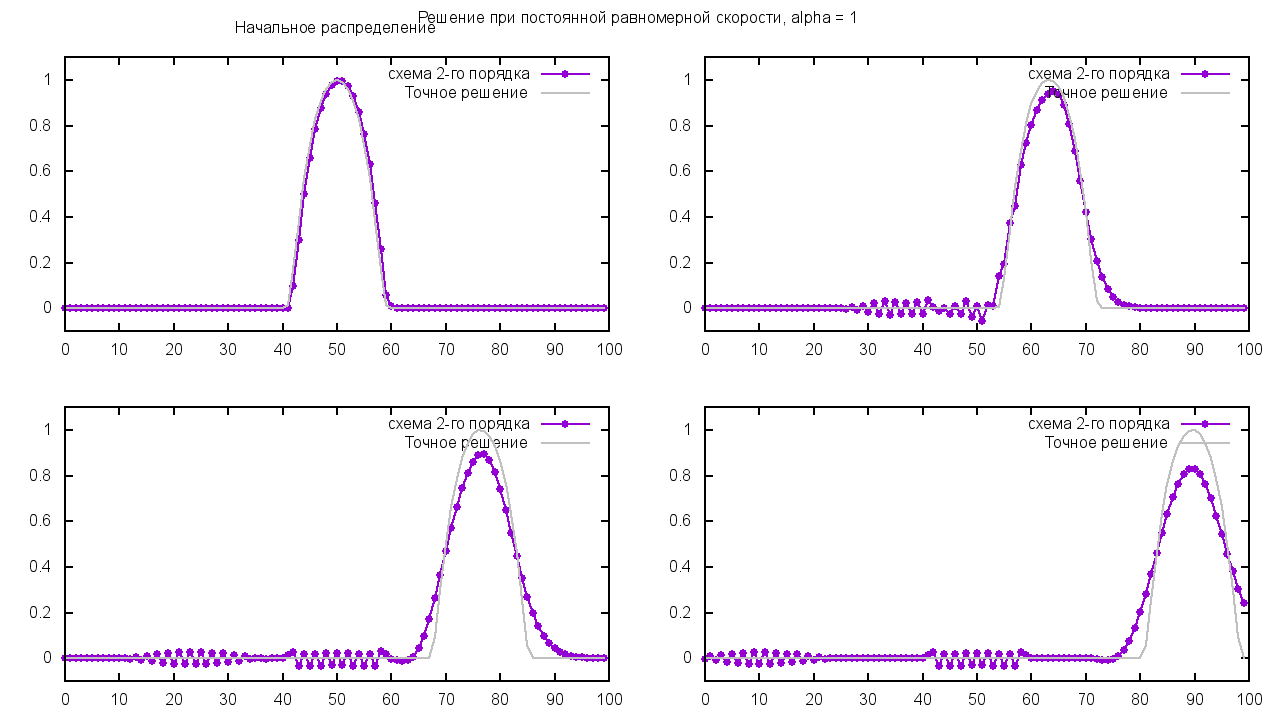
\includegraphics[width=1.2\linewidth]{pics/alpha1_notvd}
	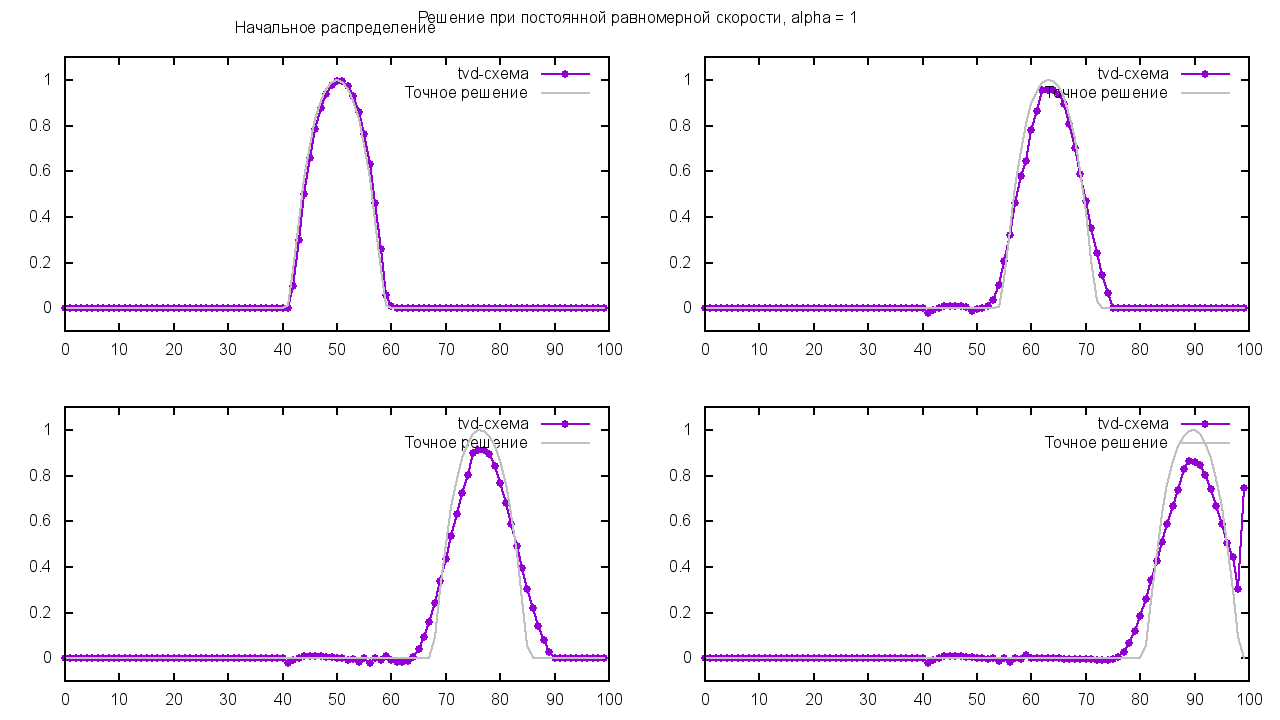
\includegraphics[width=1.2\linewidth]{pics/alpha1_tvd}
\end{figure}

Для дробного $\alpha = 0.9$ была применена та же TVD-схема, получены решения

\begin{figure}
	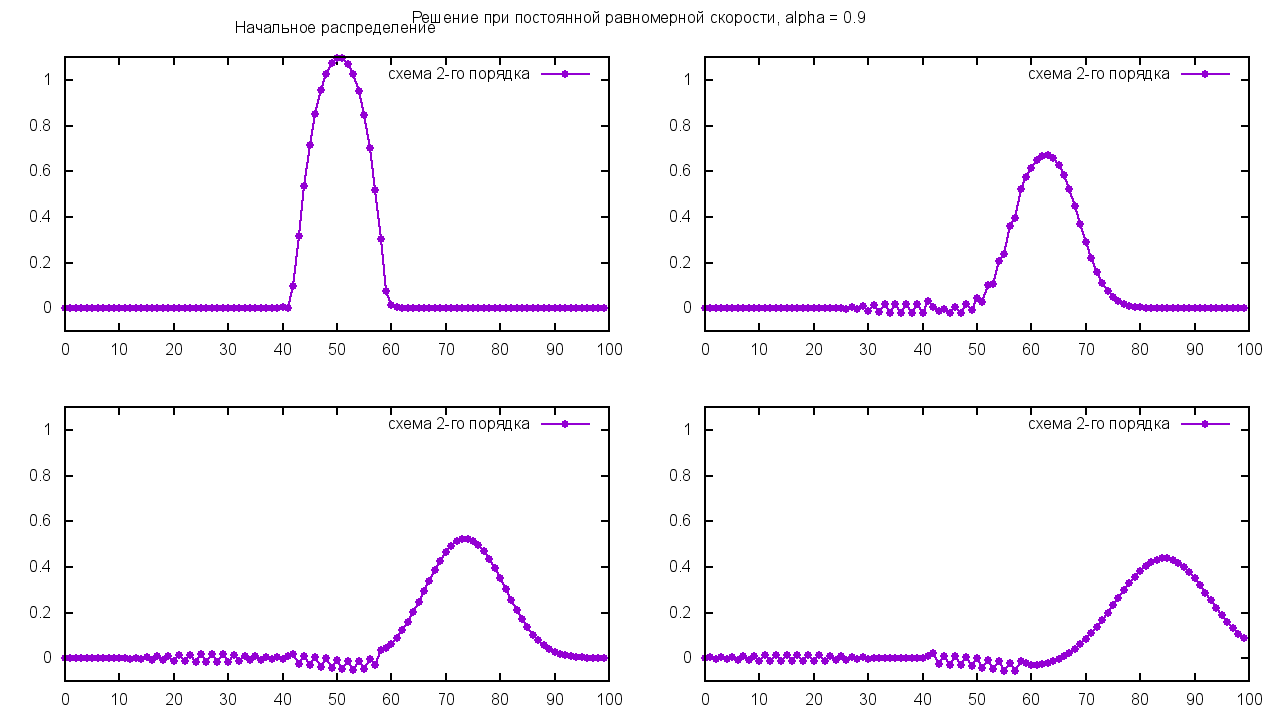
\includegraphics[width=1.2\linewidth]{pics/alpha09_notvd}
	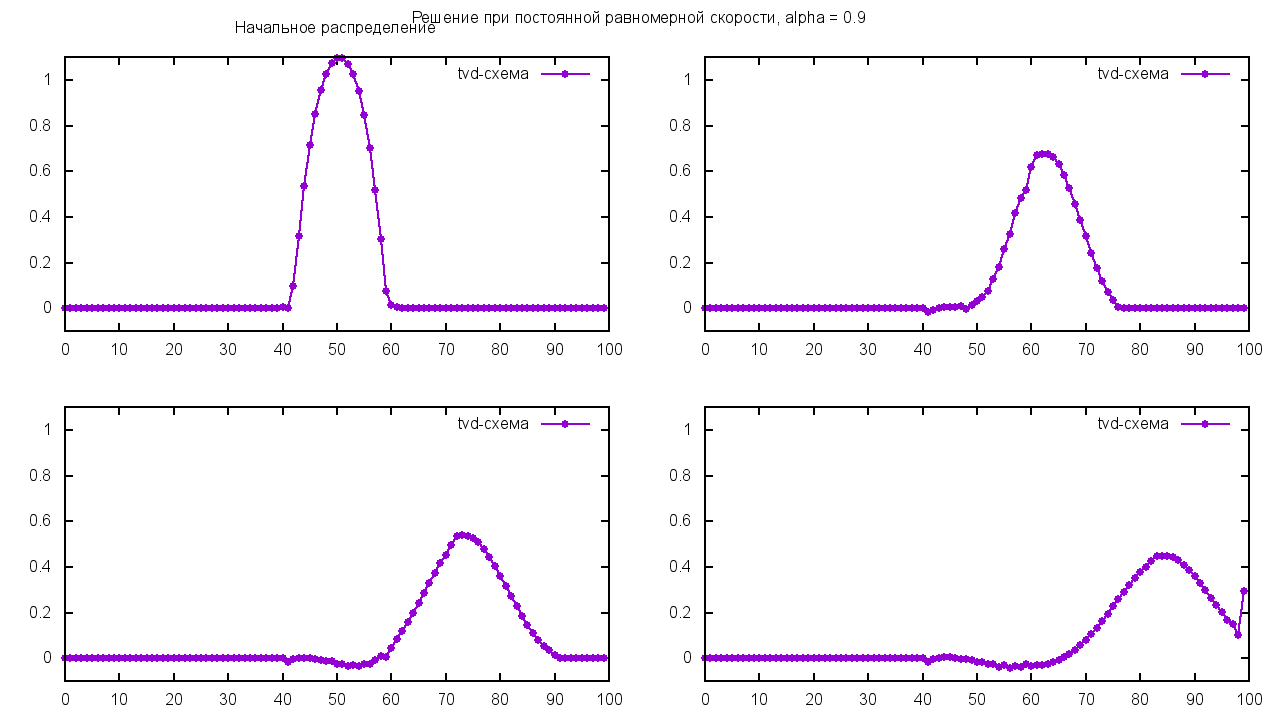
\includegraphics[width=1.2\linewidth]{pics/alpha09_tvd}
\end{figure}

Также получены решения для $\alpha = 0.7$:

\begin{figure}
	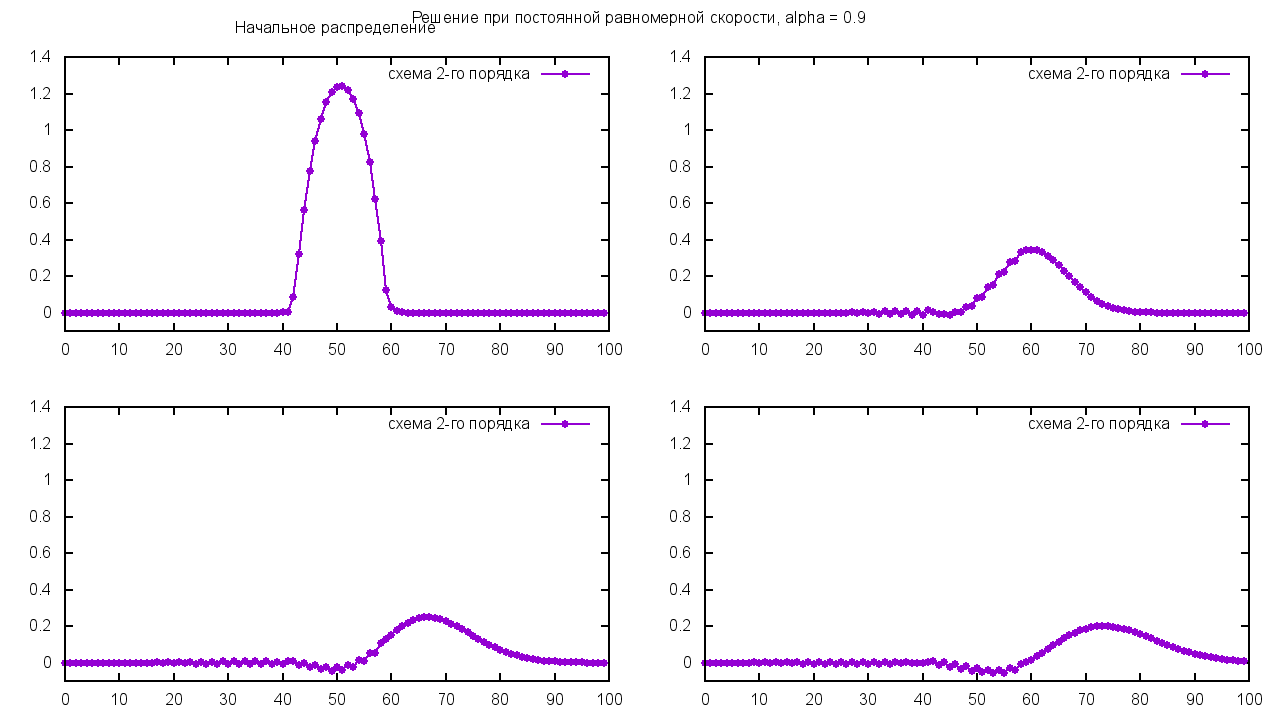
\includegraphics[width=1.2\linewidth]{pics/alpha07_notvd}
	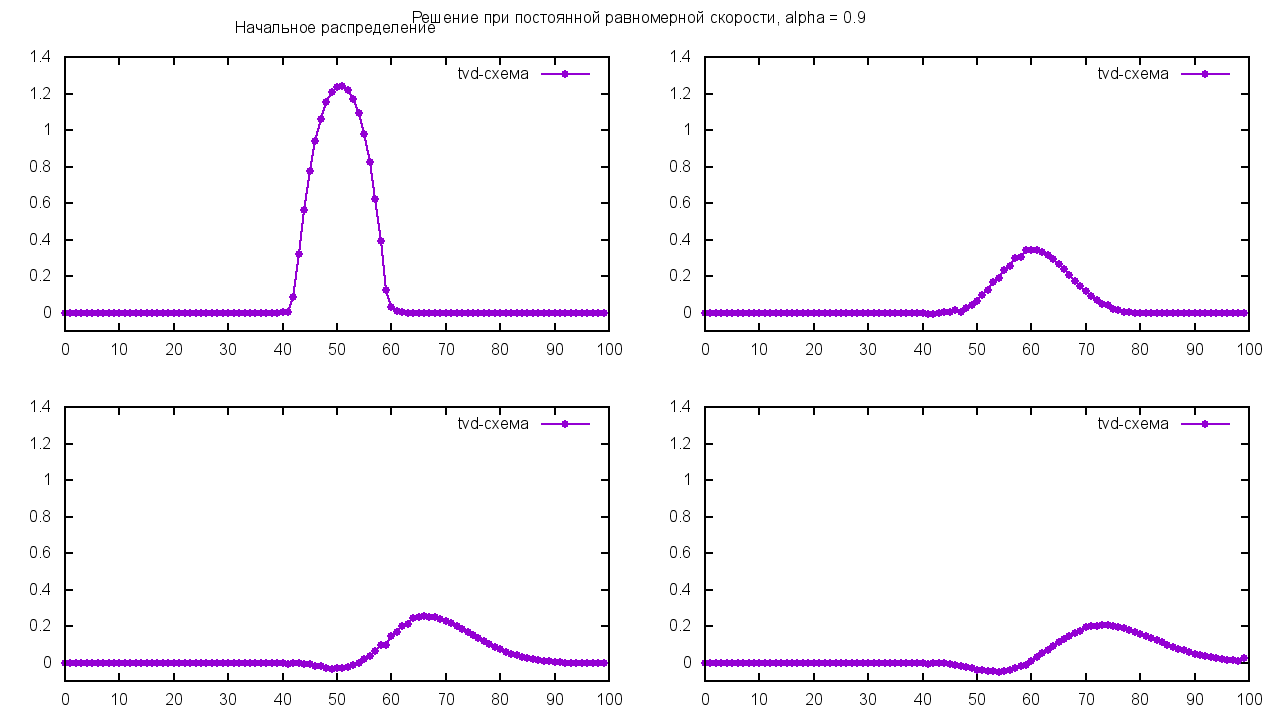
\includegraphics[width=1.2\linewidth]{pics/alpha07_tvd}
\end{figure}

Также получены решения для $\alpha = 0.5$:

\begin{figure}
	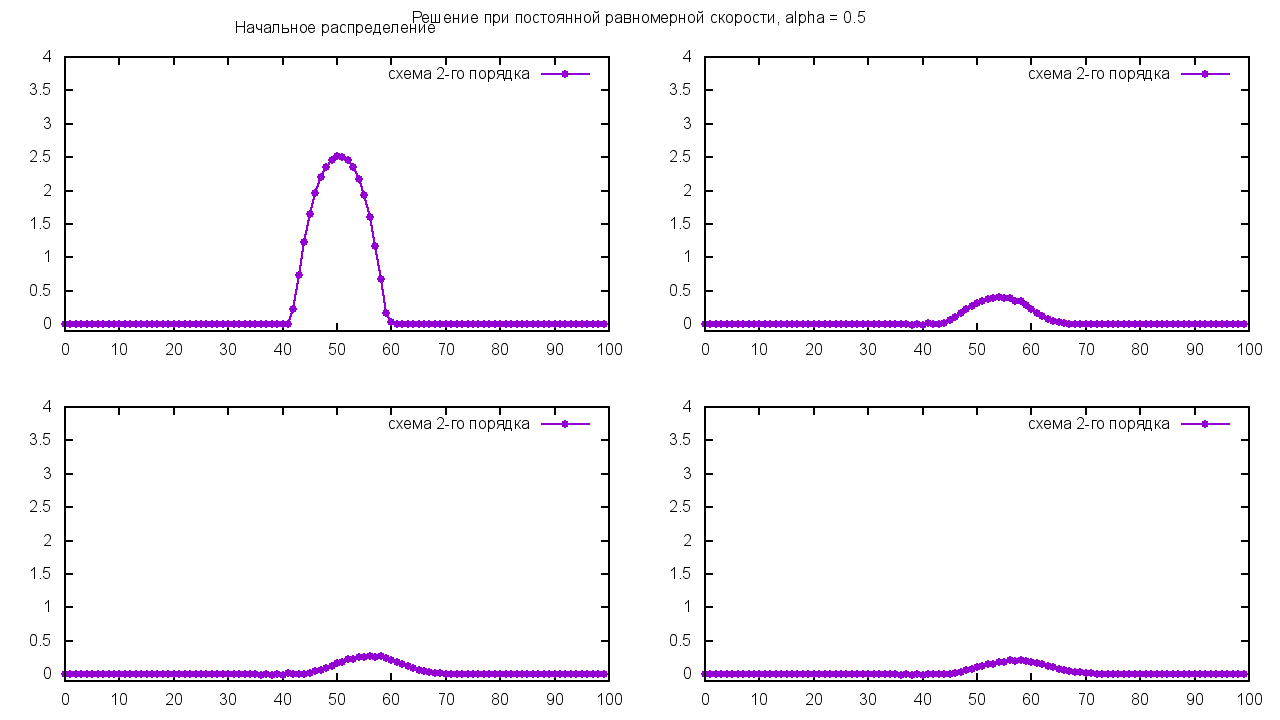
\includegraphics[width=1.2\linewidth]{pics/alpha05_notvd}
	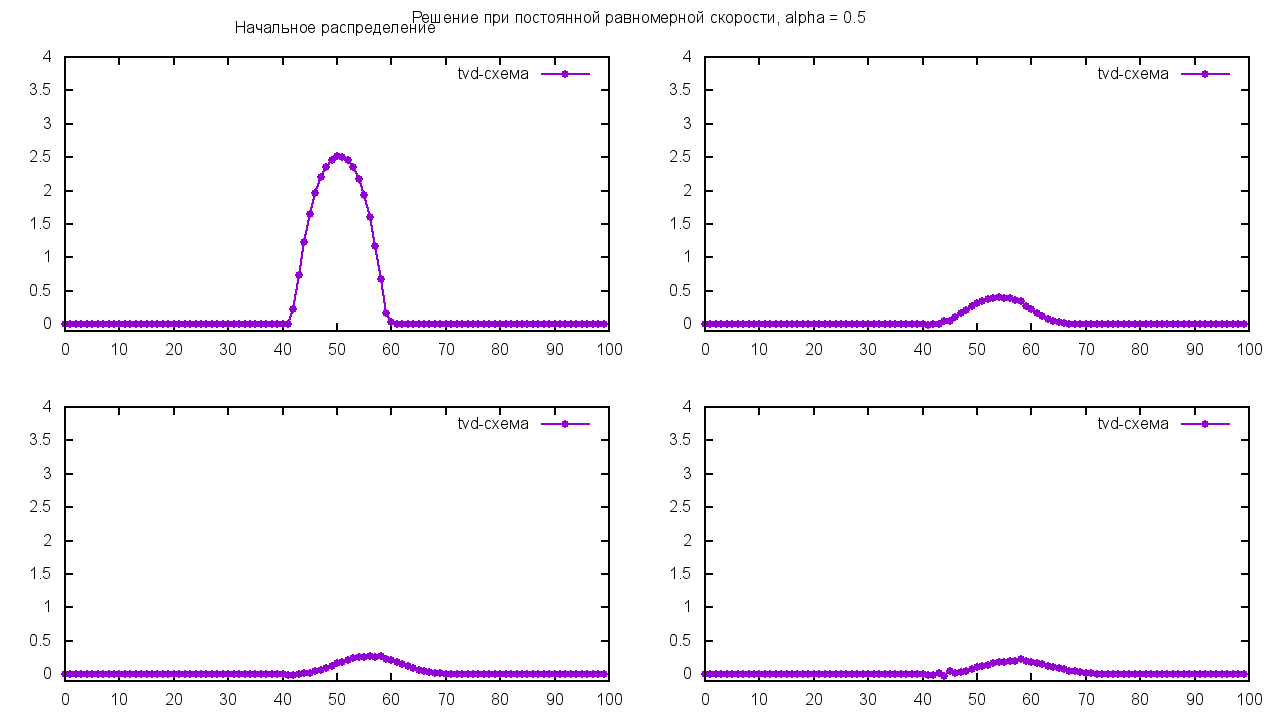
\includegraphics[width=1.2\linewidth]{pics/alpha05_tvd}
\end{figure}


%\begin{thebibliography}{99}
%	\addcontentsline{toc}{chapter}{Список литературы}
%	\input{bib.tex}
%\end{thebibliography}

\end{document}
